%
% File naaclhlt2010.tex
%
% Contact: nasmith@cs.cmu.edu

\documentclass[11pt,letterpaper]{article}
\usepackage{naaclhlt2010}
\usepackage{times}
\usepackage{latexsym}
\usepackage{amsmath}
\usepackage{tikz}
\usepackage{graphicx}
\setlength\titlebox{6.5cm}    % Expanding the titlebox


\title{Identification of Bacterial and Eukaryotic Genes using Interpolated Markov Model}

\author{Jacob Pritt\\
  {\tt mpritt4@jhu.edu}
  \And
  Guannan Ren \\
  {\tt gren3@jhu.edu}}

\date{}

\begin{document}
\maketitle
\begin{abstract}
	We present an application and analysis of the Interpolated Markov Model (IMM) for gene identification, and a comparison of IMM to fixed-length Markov models. By implementing an $8^{th}$ order IMM, we came close to replicating the results of the original GLIMMER paper for gene finding.In comparing the general Markov chain model against our IMM, we found that the interpolated Markov model outperforms the general Markov chain model on almost every organism tested. When applied to eukaryotic genomes, our IMM yielded very low accuracy due to the presence of introns in genes. We overcame this problem by implementing a Hidden Interpolated Markov Model (HIMM) for exon and intron detection. Our HIMM predictor outperformed the simpler fixed-length HMM, and correctly identified intron and exon regions with 92\% accuracy.
\end{abstract}

\section{Introduction}
\paragraph{}
In the field of computational biology, gene identification and location is important in various applications such as controlling the expression level of genes. In the scope of the project, we sought to investigate Interpolated Markov Models (IMMs) and their comparison to fixed-length Markov models. A fixed-order Markov chain uses a fixed number of preceding bases to predict the DNA sequence. For example, a 5th order Markov chain would use five previous bases to predict the next base in the sequence. Markov chain run into problems when the training data is low so that the feature vectors, in our case, DNA base combinations, are too sparsely populated to estimate the probability of a base coming after. To illustrate, a $k^{th}$-order Markov model would require up to $4^{k+1}$ probabilities to be estimated from the training data. In order to have valid estimates, there must a be a certain number of occurrences of all possible k-mers in our training data, and this is rarely the case. This leads to overfitting whenever the order of the Markov model is too high for the amount of data available. 

Interpolated Markov Models address this issue by assigning different weights to k-mer sequences of varied length depending on the number of occurrences of each k-mer within the training DNA sequence. A highly frequent k-mer occurrence receives a higher weight while a low occurrence k-mer receives a lower one. When the sample data lacks a certain occurrences for a specific length k-mer, the IMM will resort to using a combination of the shorter k-mers sharing similar prefix for classification.

GLIMMER (Gene Locator and Interpolated Markov ModelER) is a tool that uses IMMs to find the genes inside a microbial genome. In the original GLIMMER publication, the authors noted that from a test batch of hundreds of bacterial genomes, the software was able to achieve over 95\% accuracy on gene identification. For our project, we first implemented the IMM algorithm used in GLIMMER and compared our classification results with that of the publication's. We also fully analyzed the improvements of and IMM-based gene classification method over a classifier that uses a fixed-length Markov model. Next we ran our algorithm on eukaryotic genomes to examine the gene identification performances on eukaryotic species. We expected the accuracy of gene identification to drop significantly for eukaryotic genes, since eukaryotic genomes have highly complex coding sequences than that of the prokaryotes.

A Hidden Markov Model is used when a process that follows a Markov model has some emission states that mask the underlying state. For example, consider the problem of finding exons and introns in a gene sequence. While the underlying sequence of exon and intron states can be described be a Markov model, the visible states (A, C, G, and T) do not distinguish between states. HMMs can be solved using dynamic programming, as in the Viterbi algorithm.

We attempted to apply IMMs to the HMM problem of finding exons and introns in a gene sequence. We developed a Hidden Interpolated Markov Model (HIMM) that finds exons and introns more accurately than a normal HMM.


\section{Dataset Overview}

In our project, we first sought to duplicate the results obtained from the original publication of GLIMMER. We also performed a more thorough comparison of IMMs and fixed-length Markov models for ORF classification. For these experiments, we used the H. \emph{Influenzae} genome as in the GLIMMER paper. In addition to H. influenzae, we also tested our models on the H. \emph{pylori} and the E. \emph{coli} genomes. These genomes all originate from prokaryotic genomes, which do not contain introns, making them relatively easy to classify.

We also tested the accuracy of our GLIMMER implementation on eukaryotic data. For these experiments, we used the D. \emph{melanogaster} (fruitfly) genome. Finally, we implented an IMM-based Hidden Markov Model for intron detection in eukaryotic genes. We also used the D. \emph{melanogaster} genome for this part. All genomes and coding sequences were retrieved from the GenBank database.

\section{Methods}
\subsection{GLIMMER Implementation}

Interpolated Markov Models are a modification of the Markov model that use a combination of contexts of varying length to obtain higher accuracy than a Markov model with fixed-length context. Fixed-length Markov models are only accurate up to a certain context length, after which data becomes too sparse to obtain accurate probabilities for longer contexts. Interpolated Markov models make up for this shortcoming by only using longer contexts when enough training data is available to yield an accurate probability for the given context. In the worst case, an IMM will perform just as well as a normal Markov model, but in many cases it performs much better. 

Markov models are especially applicable to DNA classification because nucleotides, especially in gene regions, are often highly dependent on the nucleotides that precede them. GLIMMER uses an Interpolated Markov model to classify potential open reading frames (ORFs) as either valid genes or noncoding segments. We implemented the GLIMMER algorithm as described in the original paper (Salzberg et al. 1998). The details of the algorithm can be found in that paper, but we describe the main steps here.

\subsubsection{Training}
GLIMMER first separates the DNA sequence into six different reading frames. Genes are processed in multiples of three, or codons, and patterns arise based on position in the codon, or reading frame. Genes can also appear either in the forward direction, or reverse complemented in the genome. This gives us a total of 6 possible reading frame positions in which genes can appear.

Initially, we search the genome for genes, or ORFs, that are more than 500 nucleotides long. These segments are very likely to be true ORFs, and they form our training set. We collect kmer counts for 7 different possible contexts. These include the 3 reading frames for forward genes, 3 reading frames for reverse complemented genes, and 1 context for noncoding regions. For each context, we store a table of counts for every kmer up to the maximum length of our model. For each base in a gene, we store the kmers ending on that base in the table for the context corresponding to the reading frame of that base. For example, consider training a model with a maximum length of 3 on a gene 'ATGGCA...'. First we would increment the count for 'A' in the context for reading frame 1. Next, we would increment the counts for 'T' and 'AT' in the context for reading frame 2. Next, we would increment the counts for 'G', 'TG', and 'ATG' in the context for reading frame 3. Next, we would increment the counts for 'G', 'GG', and 'TGG' in the context for reading frame 1. By having a model for each reading frame, we can find patterns dependent on the reading frame more accurately.

\subsubsection{Classification}
For our classification step, we first generate a list of all potential ORFs, defined as sections with a length that is a multiple of 3 that begin with 'ATG' and end with one of 3 stop codons. For each potential ORF, we score it in each of the 7 contexts described above. For example, to score an ORF in reading frame 1 we would calculate the probability of the first base according to the model for reading frame 1, then multiply by the probability of the second base according to the model for reading frame 2, and so on. If the region is a true ORF for a forward gene, we would expect its score in ORF 1 to be higher than all other scores. Similarly, if the region is a true ORF for a complementary gene, we would expect its score in complementary ORF 1 to be higher than all others. If the reading frame with the highest score matches the ORFs actual reading, and the score is greater than some threshold value, we approve it as a true ORF.

To calculate the IMM score for a string $S=s_1s_2...s_n$, we must calculate a weight $\lambda$ for the current k-mer order. Let $f$ be the number of occurrences of $s_1s_2...s_{n-1}$ in the trained table. If $f>C$ for some threshold $C$, we set $\lambda=1$. Otherwise, we calculate the Chi-squared value $d$ of the probabilities of $s_1s_2...s_nt$ and the IMM scores $s_2s_3...s_n$ for each $t\in \{A,C,G,T\}$. If $d < 0.5$, we set $\lambda=0$, otherwise, $\lambda=\frac{d\cdot f}{C}$. Thus, if the frequencies for the current order are significantly different from the IMM values for the next shorter order, we prefer to use the current frequencies as a more accurate predictor.

\subsection{Iterative GLIMMER}
We attempted to improve our GLIMMER results by iteratively training and classifying multiple times. In the first iteration, we trained our IMM on long ORFs as described in the Training section above and then classified all potential ORFs. In all subsequent iterations, we trained our model on the ORFs approved by the previous classification step and then reclassified all the ORFs.

We hypothesized that the Iterative IMM would yield more accurate results than the sin\textit{gl}e-iteration IMM. We theorized that the long ORFs used to train the initial IMM might not be representative of all ORFs, and iterative training would allow us to train on a more accurate sample of the ORFs. Surprisingly, however, this was not the case. On the contrary, we found that iterative training caused our accuracy to decrease with each iteration. We abandoned this idea when we found that it didn't work.

\subsection{Exon/Intron Classification with Hidden Interpolated Markov Models}
One of the goals of our project was to use the Interpolated Markov Models to detect exon and intron regions in a gene. Unlike ORFs, which must begin with 'ATG' and end with a well-defined stop codon, introns may begin and end at arbitrary points in a gene. Thus, we had to construct a Hidden Markov Model (HMM) using the interpolated context. We call this model the Hidden Interpolated Markov Model (HIMM). HIMMs have already been used for gene detection (Salzberg et al. 1999), but we did not refer to any of these papers and developed this model on our own.

A Hidden Markov Model is used when a process follows a Markov model but the current state of the model is hidden by extra emission states. In our application, the DNA might be in an intron or an exon at any time, but in either case will only output 'A', 'C', 'G' and 'T'. Figure 1 shows the Markov model for this problem. Note that while in an exon, the reading frame will increase by 1 at every base. The gene may enter an intron from any reading frame, but when it reenters and exon it must resume in the same reading frame where it left. We adapted the Viterbi algorithm, which uses dynamic programming, along with our interpolated model to solve this problem.

\begin{figure}
	\begin{center}
		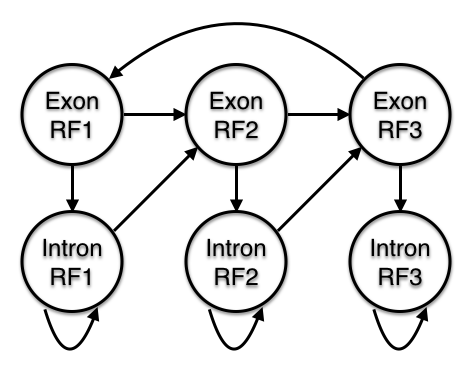
\includegraphics[scale=0.4]{HMM.png}
	\end{center}
	\caption{\label{font-table} Hidden Markov Model for exons and introns.}
\end{figure}

\subsection{Training}
We trained a total of 10 models on 4 different states (orf1, orf2, orf3, intron). These models include: orf1 $\rightarrow$ orf2, orf2 $\rightarrow$ orf1, orf3 $\rightarrow$ orf1, each of the orfs  $\rightarrow$  intron, intron  $\rightarrow$ each of the orfs, and intron  $\rightarrow$  intron. The 3 intron states are all identical (hence why we combined them into a single state here) but we must represent it as 3 states when calculating our model to enforce the reading frame constraint. For each model, we count all the kmers of every length up to the maximum such that the first k-1 bases lie in the first state and the last base lies in the second state.

We trained our model on 10\% of the genes from our dataset and tested on the remaining 90\%.

\subsection{HIMM}
We used dynamic programming to implement our HIMM. We first construct an empty matrix with 6 rows (one for each state) and a column for each base in the gene to be modeled. We then fill this matrix column by column such that $M_{i,j}$ contains the log-probability of the most likely path from the beginning of the gene to state i for base j. For each state, there are only 2 possible states that can precede it as shown in Figure <<reference>>. We use the Interpolated Markov Model to determine the most likely new state given the preceding kmer and the kmer counts from the training step. The new probability is equal to

$$M_{ij} = \max_{k \in states} M_{k,j-1} \cdot Pr\left({S_\ell}_i \mid \left( S_1,...S_{\ell-1}  \right)_k \right)$$

 In parallel with filling in the probability matrix, we fill in a backtrace matrix of the same dimensions that stores the backtrace of the most likely path from each state to $M_{0,0}$. After completing both matrices, we simply find the highest value in the last column of the probability matrix and follow the backtrace from the corresponding cell in the backtrace matrix.



\section{Results}

We used the complete H. \emph{influenzae} genome to evaluate the performance of our IMM gene classifier. We ran the IMM algorithm for varying maximum k-mer length from 0 to 9. A maximum k-mer length of 0 indicates that predictions are made with no information about the preceding nucleotides, while a maximum k-mer length of 9 indicates that the current nucleotide’s probability is dependent upon at most 9 preceding DNA nucleotides. We also implemented and tested a fixed-length Markov chain model to compare to IMM results at each k-mer length. The fixed-length Markov model is trained and tested identically to the IMM, but always assigns a weight of 1 to the longest k-mer length, so it never uses any other k-mer lengths. Both models also used +1 smoothing to reduce overfitting.

\subsection{Comparison of IMM and Markov chain on H.influenzae data}
Figure 2 shows how the IMM compares against the Markov chain model at identification of H. \emph{influenzae} genes for varying model complexity. As we would expect, the fixed-length Markov model begins to lose accuracy for $k>6$, while the IMM accuracy never decreases when k-mer length increases. Interestingly, the fixed-length model has strong peaks for k-mers that are multiples of 3. This is likely an artifact resulting from the 3-mer-based structure of genes.

\begin{figure}
	\begin{center}
		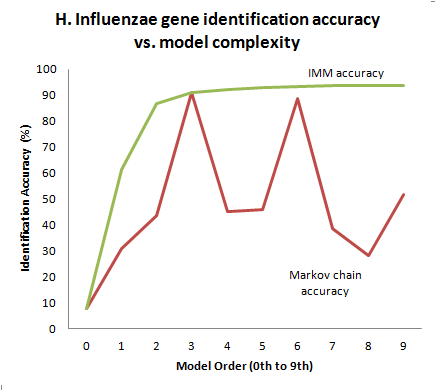
\includegraphics[scale=0.8]{plots/accuracy_vs_model_complexity.png}
	\end{center}
	\caption{\label{font-table} Accuracy comparison for IMM and MC models at different model complexity for \emph{H. influenzae} genome}
\end{figure}

We also recorded the running time (Figure 3) and number of false positives (Figure 4) for both models for varying k-mer length. 

\begin{figure}
	\begin{center}
		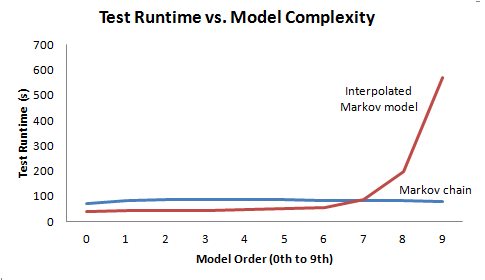
\includegraphics[scale=0.8]{plots/runtime_vs_model_complexity.png}
	\end{center}
	\caption{\label{font-table} Runtime comparison for IMM and MC models at different model complexity}
\end{figure}

\begin{figure}
	\begin{center}
		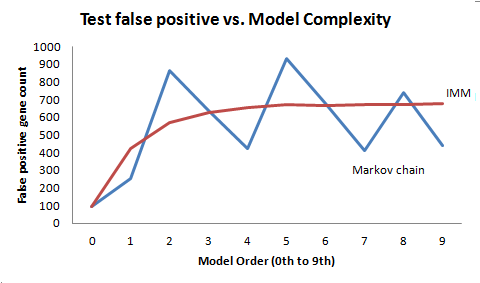
\includegraphics[scale=0.8]{plots/false_positives_vs_model_complexity.png}
	\end{center}
	\caption{\label{font-table} False positive gene identified for IMM and MC models at different model complexity}
\end{figure}

We were interested to see how our model generalize to other bacterial genomes, so we ran similar tests on H. pylori and E. coli genomes. The comparisons between an $8^{th}$ order interpolated Markov model and an $8^{th}$ order Markov chain for different prokaryotes are shown in Table 1.

\begin{table}
	\begin{center}
		\begin{tabular}{|c|c|c|}
			\hline \bf Organism & \bf MC Acc.(\%) & \bf IMM Acc.(\%) \\ \hline
			H. influenzae & 51.87 & 93.87 \\
			\hline
			H. pylori & 44.47 & 96.88 \\
			\hline
			E. coli & 27.92 & 58.79 \\
			\hline
		\end{tabular}
	\end{center}
	\caption{\label{font-table} Generalization of Markov chain and interpolated Markov model to other prokaryotic genomes at $8^{th}$ order complexity}
\end{table}


\subsection{Gene finding on Eukaryotic organisms}

While not mentioned in the original GLIMMER publication, gene identification on Eukaryotic genome sequences using the IMM is something we set out to test. Using the complete genome for Drosophila melanogaster’s chromosome X, we ran our IMM and fixed-length Markov chain algorithms to yield the results as shown in Figure 5. The IMM model yields very poor accuracy on this data. This result is expected, since Eukaryotic genomes are much more complex than those of Prokaryotes. For example, the extra non-coding intron sequences and the regulatory sequences such as promoters and enhancers increase the noise which our gene identifier has to go through. 

\begin{figure}
	\begin{center}
		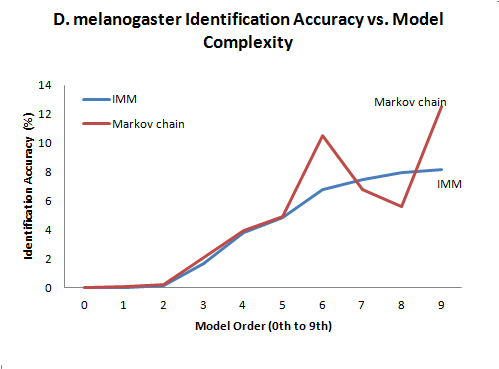
\includegraphics[scale=0.8]{plots/accuracy_vs_model_complexity_drosophila.png}
	\end{center}
	\caption{\label{font-table} Accuracy comparison for IMM and MC models at different model complexity for \emph{D. melanogaster} genome}
\end{figure}


\subsection{Gene finding with Hidden interpolated Markov Models}

Figure 6 compares the accuracy results for the HIMM and the normal HMM for exon and intron detection. These results were gathered from the D. melanogaster genome. Both models were trained on 10% of the genes and tested on the remaining 90%.

\begin{figure}
	\begin{center}
		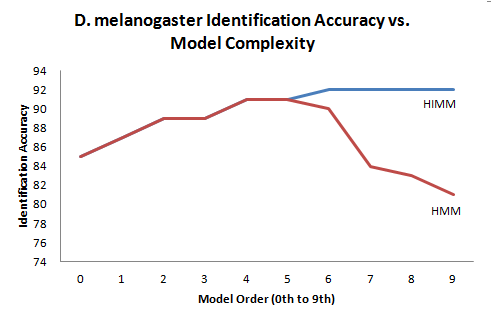
\includegraphics[scale=0.8]{plots/accuracy_vs_model_complexity_drosophila_hmm.png}
	\end{center}
	\caption{\label{font-table} Accuracy comparison for HIMM and HMM models at different model complexity for \emph{D. melanogaster} genome}
\end{figure}



\section{Discussion}

When comparing our $8^{th}$ order IMM results against the same model as used in the publication, we noticed that our accuracy value of 93.78 \% differs significantly from the accuracy of 97.8 \% reported. This is likely due to a difference in datasets used. The GLIMMER paper reported using not only annotated genes, but experimentally-generated results as well. In contrast, our data was drawn only from GenBank annotations. This theory is supported by the fact that the GLIMMER publication reported using 1717 confirmed genes while our annotation file contained only 1174 genes. The difference in the number of annotated genes largely affect the number of false positive ORFs in our results, which is significantly higher than reported in the GLIMMER paper.

We noticed something interesting from the fixed-length Markov chain results that is not apparent in the IMM results. The identification accuracy of the fixed-length Markov chain peaks at intervals of three bases. We think that this might be due to the fact that codons are coded by 3 bases. 

Overall, we are satisfied with the accuracy of our IMM on the identification of true bacterial genes.

Based on the results from our IMM gene finder for prokaryotic genomes, we were less thrilled when we tested our IMM on the eukaryotic D. \emph{melanogaster} genome. At an $8^{th}$ order model complexity, we only have a gene identification accuracy of 7.97 \% for the IMM. This extremely low accuracy is largely due to the presence of introns in eukaryotic genes.

Using our HIMM approach, we were able to detect these exon and intron regions with very high accuracy. At a $8^{th}$ order model, exon identification with the HIMM is roughly 92 \%. 

Once again, we compared the standard fixed-length HMM model to our new HIMM model. As we expected, just in our gene identification algorithm, accuracy begins to decrease past the $6^{th}$ order HMM due to the feature sparsity problem. As discussed for the IMM, the HIMM alleviates this problem by weighing in shorter k-mer length sequences preceding the current nucleotide and achieves a better result as the model complexity increases.

\subsection{Comparison to Project Proposal}
Judging by our original project proposal, we have accomplished the must-achieve milestones by implementing an IMM classification program closely following the program specifications of the GLIMMER publication. We have also managed to finish the features mentioned in the expected to achieve section. We have written a Markov model to compare the results obtained to that of the IMM’s. Surprisingly, we have also accomplished our original reach-goals for looking into  approaches to optimize the IMM’s accuracy. While the iterative approach was unsuccessful in increasing accuracy, we successfully implemented a Hidden IMM algorithm that was able to identify introns with high accuracy. We extended beyond our original plans by implementing a Hidden interpolated Markov Model for eukaryotic gene finding.
An idea for future work for this project would be to look at GLIMMER2.0 and try to implement an interpolated context model that decides which positions to use for prediction.


\begin{thebibliography}{}

\bibitem[\protect\citename{Salzberg, S.L., Delcher, A.L., Kasif, S. and White, O.}1998]{Salzberg:98}
Salzberg, S.L., Delcher, A.L., Kasif, S. and White, O.
\newblock 1998.
\newblock {\em Microbial gene identification using interpolated Markov models}
\newblock Nucleic Acids Research: Oxford University Press.

\bibitem[\protect\citename{Salzberg,S.L., Pertea,M., Delcher,A.L., Gardner,M.J. and
	Tettelin,H.}1999]{}
Salzberg,S.L., Pertea,M., Delcher,A.L., Gardner,M.J. and
Tettelin,H.
\newblock 1999.
\newblock {\em Interpolated Markov models for eukaryotic
	gene finding}
\newblock Genomics, 59, 24–31.

\bibitem[\protect\citename{Henderson, J., Salzberg, S.L., and Fasman K.}1996]{}
Henderson, J., Salzberg, S.L., and Fasman K.
\newblock 1996.
\newblock {\em Finding Genes in DNA with a Hidden Markov Model}
\newblock Journal of Computational Biology.

\end{thebibliography}

\end{document}
